\documentclass[conference]{IEEEtran}
\IEEEoverridecommandlockouts
% The preceding line is only needed to identify funding in the first footnote. If that is unneeded, please comment it out.
\usepackage{cite}
\usepackage{amsmath,amssymb,amsfonts}
\usepackage{algorithmic}
\usepackage{graphicx}
\usepackage{textcomp}
\usepackage{xcolor}
%\usepackage[left=1.0cm,right=1.0cm]{geometry}
\usepackage{blindtext}
\usepackage{subfigure}
\usepackage{diagbox}
\usepackage{booktabs}
\usepackage{threeparttable}
\def\BibTeX{{\rm B\kern-.05em{\sc i\kern-.025em b}\kern-.08em
    T\kern-.1667em\lower.7ex\hbox{E}\kern-.125emX}}
    
\graphicspath{{figures/}}

\begin{document}

\title{HydraMini: An FPGA-based Affordable Research and Education Platform for Autonomous Driving}

\author{\IEEEauthorblockN{Tianze Wu\IEEEauthorrefmark{1}\IEEEauthorrefmark{4}, Yifan Wang\IEEEauthorrefmark{1}\IEEEauthorrefmark{4}, Weisong Shi\IEEEauthorrefmark{2}, Joshua Lu\IEEEauthorrefmark{3}}
\IEEEauthorblockA{\IEEEauthorrefmark{1}SKL of Computer Architecture, Institute of Computing Technology, CAS, Beijing, China}
\IEEEauthorblockA{\IEEEauthorrefmark{2}Department of Computer Science, Wayne State University, Michigan, USA}
\IEEEauthorblockA{\IEEEauthorrefmark{3}Xilinx, Shanghai, China}
\IEEEauthorblockA{\IEEEauthorrefmark{4}University of Chinese Academy of Sciences, Beijing, China}
{\{wutianze, wangyifan2014\}}@ict.ac.cn, weisong@wayne.edu, joshual@xilinx.com}

\maketitle

\begin{abstract}
Autonomous driving is a hot topic currently, many companies and research institutions have put a lot of effort into the topic. However, it's difficult for normal researchers or students to afford a car that is used to help them understand and do research in the area. And we believe that only when more people have the chance to make contributions then this area would be more prosperous. So in this paper, we present HydraMini, an affordable experimental research and education platform for autonomous driving. 

HydraMini is based on Xilinx PYNQ-Z2 and uses the power of the Deep Learning Processing Unit (DPU) in FPGA to accelerate the inference process. It's a full-stack platform that almost anyone is able to find their research interests and its high flexibility makes it easy to be extended or modified. It also provides useful tools like a simulator for training and testing in a virtual environment to facilitate the use of HydraMini. Our platform will help researchers and students who want to try autonomous driving or hardware accelerating build their own solutions and test it efficiently. We hope HydraMini meets three requirements: affordable, easy to understand and easy to use.
\end{abstract}

%\begin{IEEEkeywords}
%Autonomous Driving, Machine Learning, PYNQ-Z2, Field programmable gate arrays, Deep Learning Processing Unit
%\end{IEEEkeywords}

\section{Introduction}
With the development of AI technology, many work are done by robot instead of human. Driving is one of these tasks and autonomous driving(AD) has become more and more popular these years. It's obvious that AD technology will be one of the hottest topics of AI. The reason why this topic is so hot is that AD is not one single technology, but rather a highly complex system that consists of many sub-systems\cite{liu2017creating}. Nowadays, a well-performed AD car usually has multiple sensors like GPS, lidar and camera to perceive the world around it. The huge amount of sensing data generated is transferred into the computer to do processing, then the location and some other information are calculated to help the car makes decisions all by itself. AD is the area where any researcher is able to find their research interests and make contributions.

\begin{figure}[t]
    \centering
    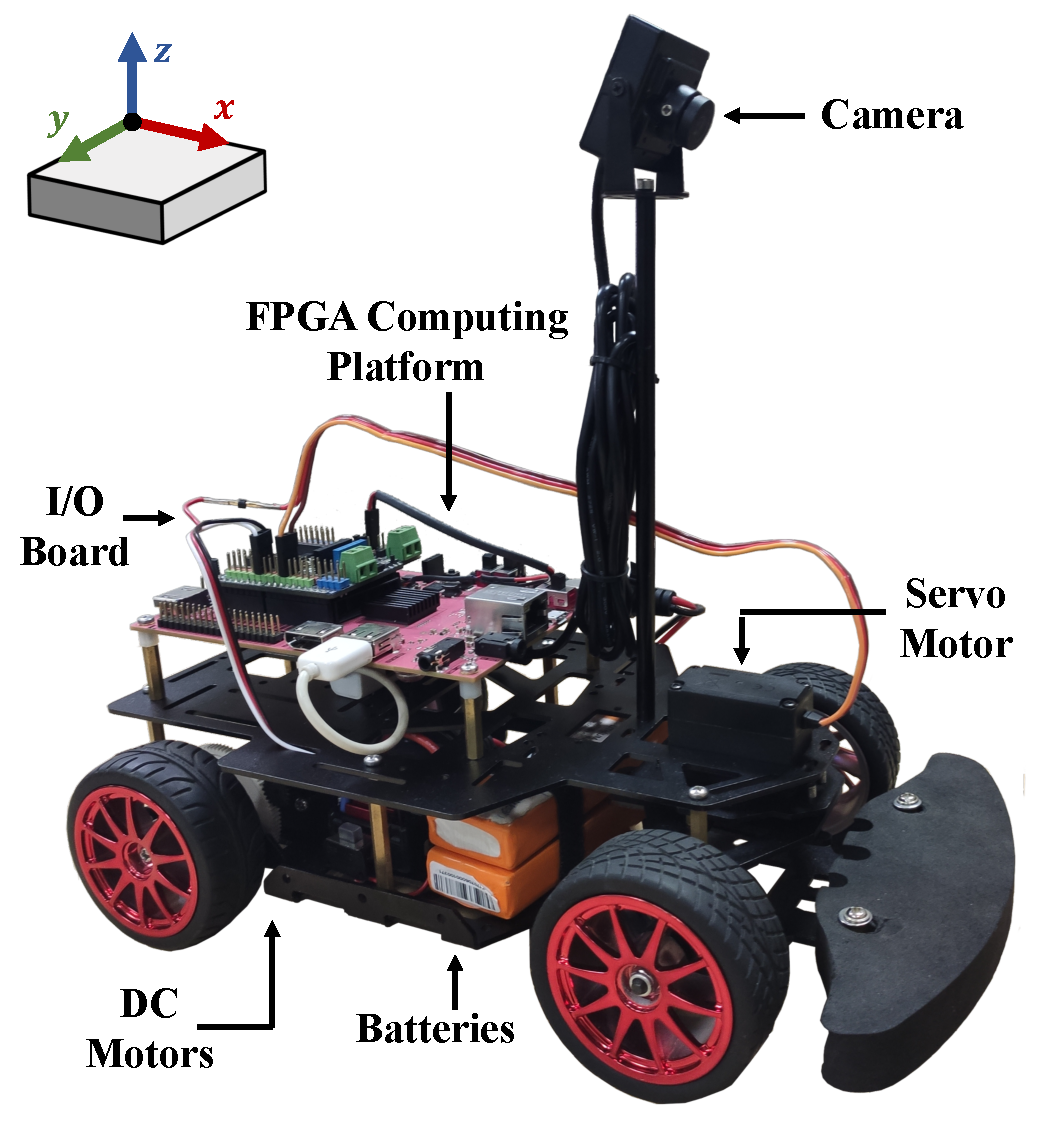
\includegraphics[width=2.5in]{hydramini}
    \caption{Overview of HydraMini Platform.}
    \label{fig:hydramini}
\end{figure}

Since there will be more people trying to learn about AD technology, a platform for AD researching and learning is badly needed. As we all know that in the cloud computing domain, researchers usually want to own machines that have good computation performance. The data center based on virtualization technology\cite{nurmi2009eucalyptus} and distributed computing\cite{dean2008mapreduce} nowadays usually has many powerful servers for data processing. And for AD tasks which are usually run in edge side, the importance of good performance is just the same as in cloud computing. The acceleration of the inference process through hardware is becoming more and more common and indispensable, it's the cornerstone of the development of AD and all the researchers and students should pay enough attention to it. However, when it comes to edge computing\cite{shi2016edge}, we should care about not only the computing power but also the power consumption and cost. It's a pity that we can hardly find one product that provides both enough computing power and hardware acceleration but remains affordable for most of the people.

\begin{table*}[t]
\centering
\caption{Platform Comparison.}
\label{tab:comparision}
\begin{tabular}{l|cccc} 
\hline
Features & Donkey Car & F1/10 & HydraOne & HydraMini \\ \hline
\hline
Computing Board & Raspberry Pi & NVIDIA Jetson TX1/TX2 & NVIDIA Jetson TX2 & Xilinx PYNQ-Z2 \\
Compputing Architecture & CPU & CPU + GPU & CPU + GPU & CPU + FPGA \\
Camera & Monocular $\times 1$ & Monocular $\times 1$ + Deep $\times 1$ & Monocular $\times 2$ & Monocular $\times 1$ \\
LiDAR & - & 2D LiDAR $\times 1$ & 3D LiDAR (16 Laser Units) $\times 1$ & - \\
Resource Management Model & - & Publisher/Subscriber (ROS) & Publisher/Subscriber (ROS) & Producer/Consumer \\
Typical Cost & $\sim\$200$ & $\sim\$2,400$ & $\sim\$1,500$ (w/o LiDAR) & $\sim\$200$ \\ \hline
\end{tabular}
\end{table*}

To make everyone have the opportunity to participate in the research of AD, we propose HydraMini, an affordable indoor experimental research and education platform for AD. It's concise and powerful, users could both learn easily and have an in-depth study. The platform was first designed for the design competition of FPT 2019\cite{wu2019end}, in this competition competitors need to build an AD car which has the abilities to finish common tasks in AD area like run along the road, avoid obstacles, understand meanings of traffic lights and so on. After attending the competition, we find the potential of our design and decide to make the project a common platform for researchers and students. As shown in Fig.~\ref{fig:hydramini}, HydraMini is a powerful and flexible platform from hardware to software. It depends on three main components: mechanical component, control system and FPGA accelerator which are the basic of modern AD technology.

We have built several study cases based on HydraMini, people are able to try AD car in a traditional way which uses computer vision methods to follow the road and do some pattern recognition, or they apply an end-to-end AI model to generate control commands directly. Also we accelerate the inference process of YoloV3\cite{redmon2018yolov3} and make it fast enough to work in a limited edge device. What's more, if your research project is based on  ROS\cite{quigley2009ros} which is widely used in robots all over the world, the migration of your project to HydraMini is easy, and with the support of functions of our platform you will probably come up with more exciting ideas. Besides, we provide tools for users, one of them is a simulator using Unity3d\cite{2019unity3d} based on sdsandbox\cite{sdsandbox} that makes the users test their design more conveniently. All the resources on HydraMini are managed by PYNQ-Z2\cite{tul2019tulpynqz2} system which is based on Ubuntu 18.04. 

Users use the computing power in PYNQ-Z2 includes both Zynq7020 FPGA\cite{zynq} which is used as a specialized hardware accelerator and an Arm 32-bit core ARM Cortex-A9 which is familiar to normal people. We believe that in the future the hardware acceleration will become an imperative for the modern cars to provide edge computing power, so it's necessary to embed FPGA which is flexible for researching in our platform. Users will find it easy to do research on multi-area of AD and develop their own algorithms and systems based on HydraMini.

The remainder of this paper is organized as follows. In Section Ⅱ, we discuss the related work. Section Ⅲ introduces the design and implementation details of HydraMini. In Section Ⅳ, we summarizes three key characteristics of our platform. We provide several case studies to show the large potential of HydraMini in Section Ⅴ. Finally, we conclude our work in Section Ⅵ.
\section{Related Work}
In this section, we summarize the related work and several other similar platforms. Compared to above products, our platform costs less and provides FPGA support, also it's easy for users to custom their own components based on it. The basic of our tool kit is simple and affordable, but it has great potential. \textbf{Table 1} shows the comparison between these platforms.

\textbf{Research Platform for Autonomous Devices.} Wang et al. presented HydraOne\cite{wang2019hydraone}, HydraOne is an indoor robot-based platform, it has sufficient resources and components to conduct related experiments. It has three key characteristics: design modularization, resource extensibility and openness, as well as function isolation, which allows users to conduct various research and education experiments. Wei et al. presented the CMU autonomous driving research platform which is based on a Cadillac SRX\cite{wei2013towards}. This work focuses on vehicle engineering problems, including the actuation, power, and sensor systems on the vehicle. Matthew O’Kelly et al present F1/10\cite{o2019f1}: an open-source, affordable, and high-performance 1/10 scale autonomous vehicle testbed. The F1/10 testbed carries a full suite of sensors, perception, planning, control, and networking software stacks that are similar to full scale solutions. 

\textbf{Hardware Acceleration Technology used in AI.} GPU\cite{nurvitadhi2016accelerating} is now widely used by researchers to accelerate the training and inference process of AI. The training library is cuDNN\cite{cudnn} while the inference library is TensorRT\cite{tensorrt}. cuDNN is a GPU-accelerated library of primitives for deep neural networks. It provides highly tuned implementations of routines arising frequently in DNN applications. TensorRT focuses specifically on running an already trained network quickly and efficiently on a GPU for the purpose of generating a result; also known as inferencing. The tensor processing unit was announced in May 2016 at Google I/O, when the company said that the TPU had already been used inside their data centers for over a year\cite{techradar}. The chip has been specifically designed for Google's TensorFlow framework, a symbolic math library which is used for machine learning applications such as neural networks.\cite{tensorprocessingunit} The Xilinx Deep Learning Processor Unit (DPU)\cite{dnndk} is a programmable engine optimized for convolutional neural networks. The unit includes a high performance scheduler module, a hybrid computing array module, an instruction fetch unit module, and a global memory pool module. The DPU uses a specialized instruction set, which allows for the efficient implementation of many convolutional neural network. With our platform, you are able to easily try DPU or FPGA to help your algorithms run better.
\section{Design and Implementation}
In this section, we introduce the design and implementation details of HydraMini. The structure of the system is shown in Fig.~\ref{fig:framework_overview}. Based on the middle ware, users are able to add more kinds of sensors or create more workers to handle the data while the middle ware provides apis for users to take advantage of computing resource and control the car. It's easy for users to add or remove component to or from the system. 

\begin{figure}[t]
    \centering
    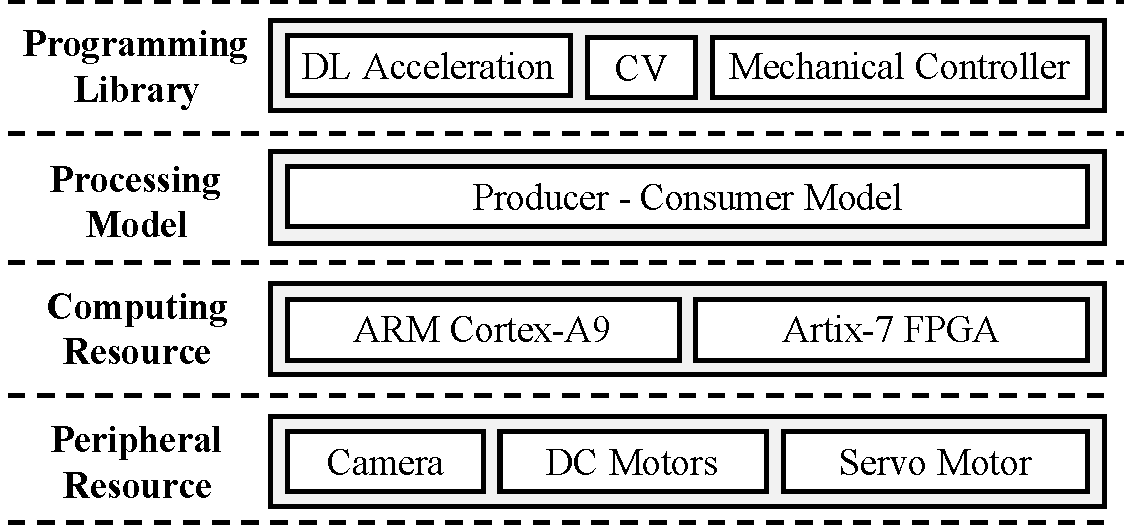
\includegraphics[width=3.25in]{framework_overview}
    \caption{HydraMini Framework Overview.}
    \label{fig:framework_overview}
\end{figure}

\subsection{Hardware Design}
As shown in Fig.~\ref{fig:hardware}, HydraMini is equipped with a Xilinx PYNQ-Z2 board which acts as the main controller, PYNQ\cite{tul2019tulpynqz2} is an open-source project from Xilinx that makes it easy to design embedded systems with Xilinx Zynq Systems on Chips (SoCs). Users create high performance embedded applications with parallel hardware execution, high frame-rate video processing, hardware accelerated algorithms, real-time signal processing, high bandwidth I/O and low latency control. Software developers will take advantage of the capabilities of Zynq and programmable hardware without having to use ASIC-style design tools to design hardware. System architects will have an easy software interface and framework for rapid prototyping and development of their Zynq design. It's suitable to be used in our platform because of the convenience and high performance. The board collects the data from multiple sensors and feeds the data to several computing tasks in real-time. An I/O expansion board V7.1 receives the control message output from the computing tasks and then sends the control signals to the motor drivers to control the movement of HydraMini. The whole HydraMini platform is powered by two Batteries. And to provide steady voltage for PK370PH-4743 motor and DF15MG electric servo motor, a QuicRun WP 1060 Brushed electronic speed controller is used. The basic sensor is one VIMICRO camera, also we provide a study case using LeiShen LS01D LIDAR. It's easy for you to add more sensors to the platform.

\textbf{Programmable Logic (PL)} The programmable logic in PYNQ-Z2 is equivalent to Artix-7 FPGA\cite{2019artix}. The components below are embedded in it:

\begin{itemize}
\item{13,300 logic slices, each with four 6-input LUTs and 8 flip-flops }
\item{630 KB of fast block RAM }
\item{4 clock management tiles, each with a phase locked loop (PLL) and mixed-mode clock manager (MMCM) }
\item{220 DSP slices }
\item{On-chip analog-to-digital converter (XADC) }
\end{itemize}

\textbf{Processing System (PS).} The Cortex-A9\cite{2019arma9} processor is embedded in PYNQ-Z2, it's a performance and power optimized multi-core processor. It features a dual-issue, partially out-of-order pipeline and a flexible system architecture with configurable caches and system coherency using ACP port. The Cortex-A9 processor achieves a better than 50\% performance over the Cortex-A8 processor in a single-core configuration. It has an L1 cache subsystem that provides full virtual memory capabilities. The Cortex-A9 processor implements the ARMv7-A architecture and runs 32-bit ARM instructions, 16-bit and 32-bit Thumb instructions, and 8-bit Java bytecodes in Jazelle state.

\begin{figure}[t]
    \centering
    \includegraphics[width=3.5in]{hardware}
    \caption{HydraMini Hardware Design.}
    \label{fig:hardware}
\end{figure}

\subsection{Software Design}
\textbf{Framework Overview.} The operating system on PYNQ-Z2 is based on Ubuntu 18.04, so libraries are easily installed. The system on PYNQ-Z2 also provides many jupyter notebook documents about how to fully utilize the hardware resources in PYNQ-Z2. To make the control process more efficient and easier to extend, we implement a producer-consumer model\cite{producerconsumer} which is a classic design pattern in multi-process synchronization environment. The whole control system depends on three main components: mechanical controller, AI model inference and computer vision analysis. 

\textbf{Producer-Consumer model.} Many indoor AD driving platforms like HydraOne\cite{wang2019hydraone} and F1/10\cite{o2019f1} use ROS\cite{quigley2009ros} to manage the hardware and software resources nowadays because ROS provides the car with an easy way to communicate with the server and many existing applications. However, to make a balance between the platform's cost and performance, we focuses mainly on core functions in AD and the communication between car and server is not so important. Using ROS will bring unnecessary overhead to CPU. So a more streamlined and efficient method is used as the base of the control system. Refer to Fig.~\ref{fig:producer_consumer} for an overview of this model.

\begin{figure}[t]
    \centering
    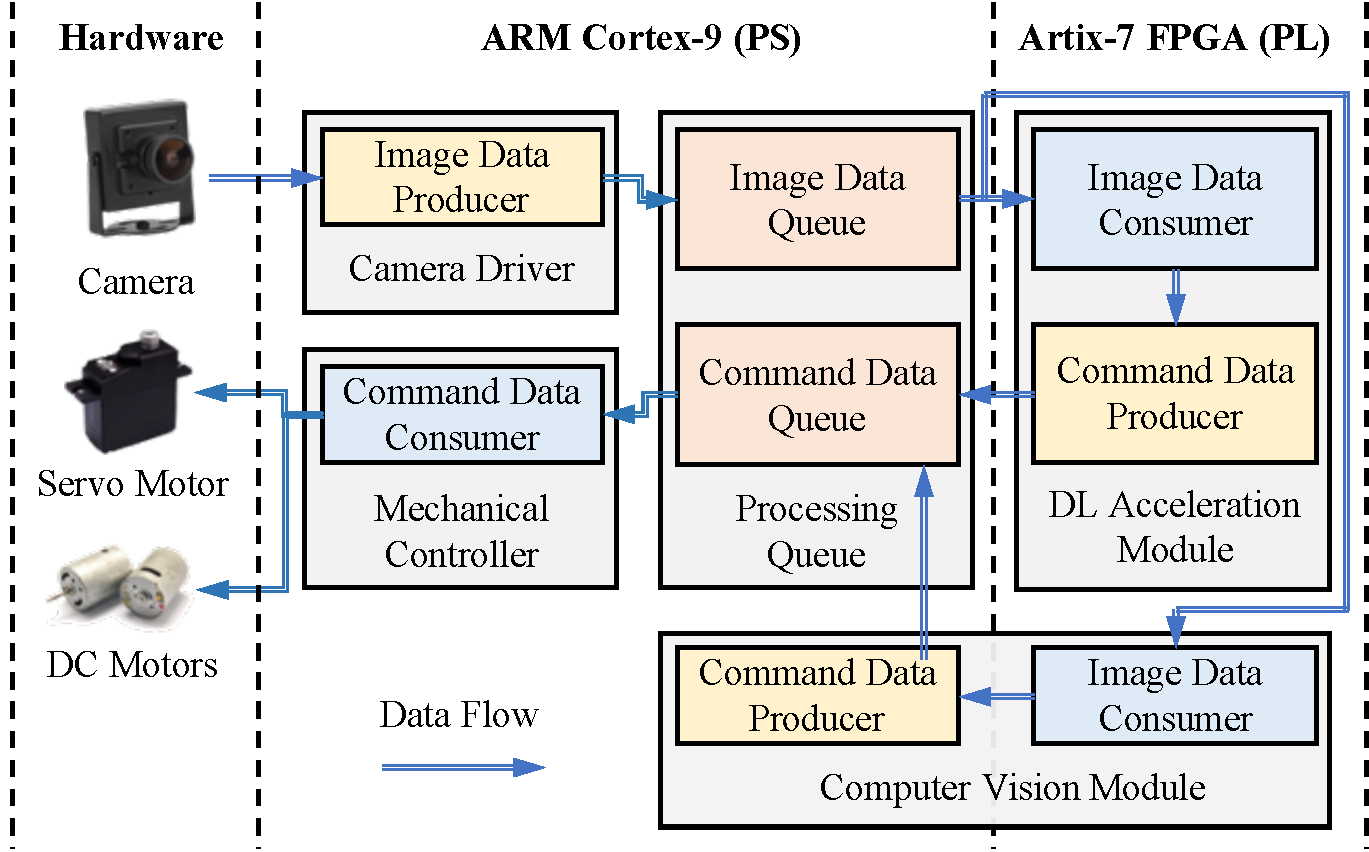
\includegraphics[width=3.25in]{producer_consumer}
    \caption{Producer-Consumer Model.}
    \label{fig:producer_consumer}
\end{figure}

The sensors like camera will play the role of producer while the decision makers like AI model and computer vision methods will be consumers. Each kind of data will be stored in a queue in memory. Different producer processes add the data they get to the specified queue and will be handled by consumers who cares about this kind of data. It's easy to add more producers or consumers and new kind of data. If one process want to handle or provide different kind of data, just read or write the related queue. The synchronism of the system is maintained by locks, each queue will have a lock.

The consumers who usually act as controller have a shared clock. They will check if their commands to send is outdated according to the clock, this clock ensures that the car won't receive outdated commands. Also, there exists a token which indicates who has the current property in control power. Users are able to define their own strategy for the transformation of property.

\textbf{Mechanical Controller.} The HydraMini platform has one motor for providing power and one servo motor for direction control. This design has been widely used in real cars. We provide basic control apis for users. The rotate speed of the motor and the angle of deflection of servo motor are set directly. Also higher level methods like accelerating are provided too. 

Besides driving on its own, the car is controlled by using the keyboard. We invoke OpenCV\cite{opencv} library to read the keyboard signals and then call the mechanical api. Users are able to define their own button layout easily. This ability is mostly used to generate training data.

\textbf{AI Inference.} AI technology is an important part in AD, it handles many tasks like objects identification, lane keeping and so on. In our platform AI inference process is packed as a consumer thread, it reads data from produced data queue and use it as the input of AI network. Then the model produces control commands directly or just provide information for controller thread to make decisions. 

And with the power of DPU\cite{dnndk} which is one accelerator in FPGA, the process of AI reference will be accelerated. The AI inference thread is copied and they run concurrently in DPU, which means higher inference performance. 

To make good use of DPU and to make the optimization process easy, we provide scripts to do a complete set of optimized tool chains provided by DNNDK, including compression, compilation and runtime. Refer to Fig.~\ref{fig:dnndk} to see the framework of DNNDK. First the Deep Compression Tool DECENT\cite{dnndk}, employs coarse-grained pruning, trained quantization and weight sharing to make the inference process in edge meet the low latency and high throughput requirement with very small accuracy degradation. Second the DNNC (Deep Neural Network Compiler)\cite{dnndk} which is the dedicated proprietary compiler designed for the DPU will map the neural network algorithm to the DPU instructions to achieve maxim utilization of DPU resources by balancing computing workload and memory access. Third the users use the Cube of Neutral Networks (N2Cube)\cite{dnndk} the DPU runtime engine to load DNNDK applications and manage resource allocation and DPU scheduling. Its core components include DPU driver, DPU loader, tracer, and programming APIs for application development.

After using DPU, the performance of end-to-end model described in case study is up to $7,000$ FPS which is fast enough to satisfy the requirement of low-latency in AD. We also test YoloV3\cite{redmon2018yolov3} model in DPU and it achieves 3 fps when detecting 80 categories of things.

\begin{figure}[t]
    \centering
    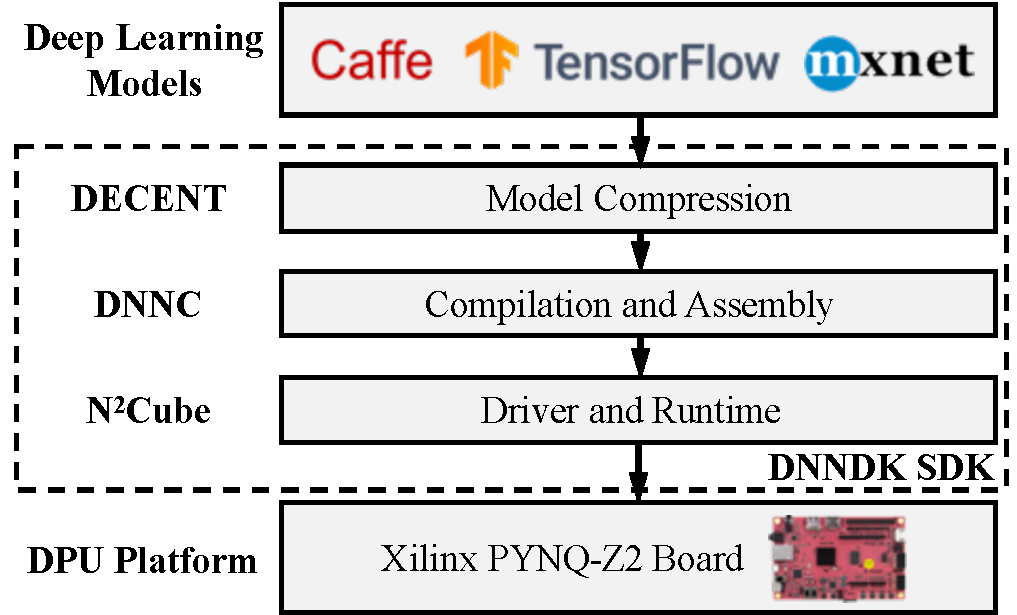
\includegraphics[width=3.25in]{dnndk.pdf}
    \caption{DNNDK Framework.}
    \label{fig:dnndk}
\end{figure}

\textbf{Computer Vision Analysis.} OpenCV\cite{opencv} is a widely used library for computer vision analysis. Due to the native support for OpenCV in PYNQ-Z2, existing computer vision algorithms are easily invoked and their own algorithms can be implemented. We have a case below which shows how to use traditional computer vision methods to manage AD tasks. The control process of these methods is just the same as AI model's, the thread running computer vision algorithms will read data from producers and output commands or information. More threads can be created to increase throughput. 

However, these computer vision algorithms may be very time consuming running in ARM Cortex-A9 in Xilinx PYNQ-Z2. To reduce computation complexity, we do several pre-process like cropping and down-sampling. Time consuming tasks such as Gaussian filter, Canny edge detection, Hough transform can be moved to FPGA using Xilinx xfopencv library\cite{xfopencv}, BP neural network can be implemented in FPGA using Xilinx Vivado HLS. However, when implementing accelerators in FPGA, users should take the board's resource into consideration and choose the heaviest computational task to implement while not beyond the resource limit. If there remains enough PL space for your algorithms, you put them in PL side, or just put them in PS side.
\section{Key Characteristics}
\begin{figure}[t]
\centering
    \subfigure[\label{subfig:end_to_end_training}End-to-End Model Training and Deployment]{
    \centering
    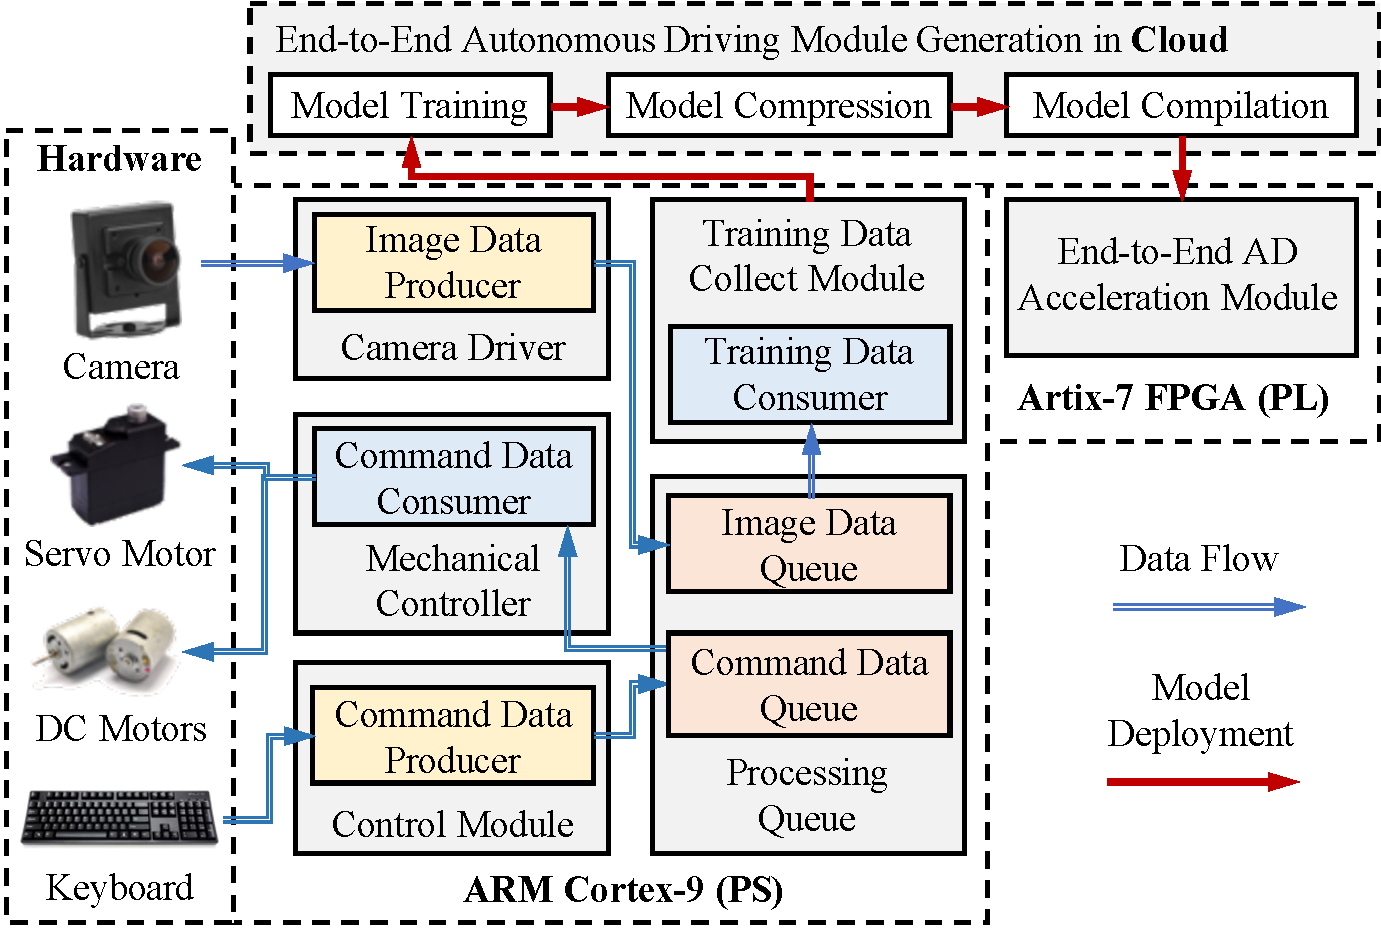
\includegraphics[width=3.4in]{end_to_end_training}
    }
    \vspace{0.1in}
    \subfigure[\label{subfig:end_to_end_inference}End-to-End Model Inference Data Flow]{
    \centering
    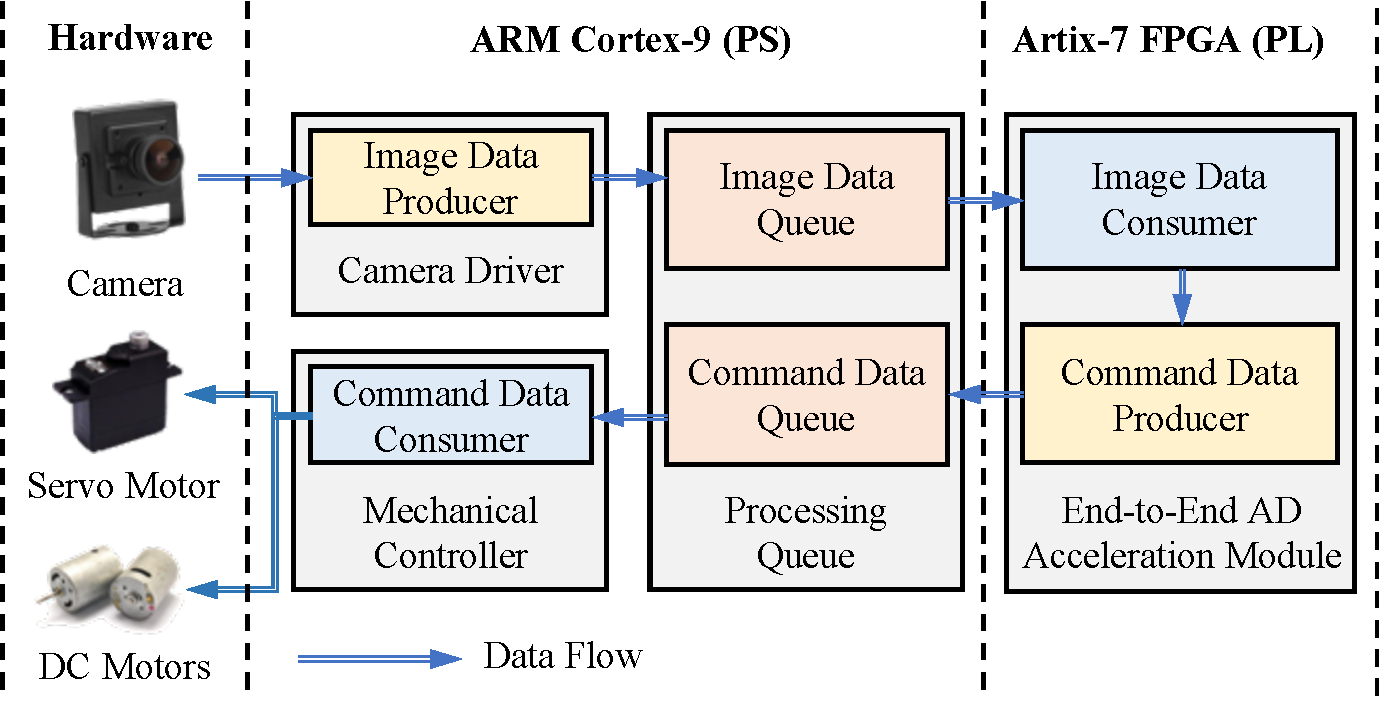
\includegraphics[width=3.4in]{end_to_end_inference}
    }
\caption{Autonomous Driving using End-to-End Model.}
\label{fig:end_to_end_autonomous_driving}
\end{figure}
The HydraMini platform has three key characteristics: high flexibility and extensibility, full stack, and easy-to-use. These three characteristics help users understand AD technology stack and the platform.

\textbf{High Flexibility and Extensibility. }The idea of our system design is inspired by ROS. In ROS, new functions are easily added by adding ROS nodes. Nodes get and send messages easily through the publish-subscribe mechanism. What we do is making the ROS system more lightweight and forthright. The thread is similar to node while the producer–consumer model is similar to the publish-subscribe mechanism. So it's easy to add more hardware devices as sensors or threads as handlers. What's more, due to the base of our system is Ubuntu18.04, it's easy to redefine the whole software framework as you like, actually we have an example of using ROS in following case studies.

\textbf{Full Stack. }The full stack here means our product provide almost everything you need to learn about AD technologies from algorithms to hardware. It's important for researchers or students to understand how the car runs and why sophisticated algorithms are able to run in resource limited edge platform. Users could use different physical construction, different operating system, different software framework, different algorithm and different hardware acceleration etc. That means researchers are able to do whatever research they want based on our platform and they could use existing modules and understand the operation mode of the whole system. Considering the difficulty users may have in collecting training data and testing AI models in real world, we provide a simulator modified from sdsandbox\cite{sdsandbox} which is first used in Donkey Car\cite{donkeycar}. The simulator is used to do tests or more. Its usage will be introduced in case studies.

\textbf{Easy-to-Use. }The most important thing we believe is to make our platform easy to use. To achieve this, most libraries of the platform are familiar to users like OpenCV and TensorFlow\cite{tensorflow}, they are open-sourced and widely used. Most importantly, the basic knowledge users should know includes only Linux, C++, Python, AI and a little about DPU usage. The software framework is simple and tidy, we only keep necessary functions and make it extendable. The hardware is simple too, if you don't want to add more devices, one camera and two motors are all you have to deal with. Users even don't have to prepare a real car to do experiments, then you care nothing about hardware. Besides, we provide many documents for users, so it's easy for them to modify any part of the platform.
\section{Case Studies}
In this section, we use four case studies deployed on HydraMini to show the capabilities of our research platform.

\subsection{Autonomous Driving using End-to-End model}
This case shows how you use our platform for AD using end-to-end model. Several recent research replaces the classic chain of perception, planning, and control with a neural network that directly maps sensor input to control output\cite{bojarski2016end, chi2017deep, eraqi2017end}, a methodology known as end-to-end driving. New approaches based on reinforcement learning are being actively developed\cite{kendall2019learning}. An end-to-end AI model is easy to use since it outputs control commands directly. The model contains mainly CNN and Dense layers\cite{keras}, it maps camera input to control output. The structure of the model is shown in Fig.~\ref{ms}.

\begin{figure}[b]
\centerline{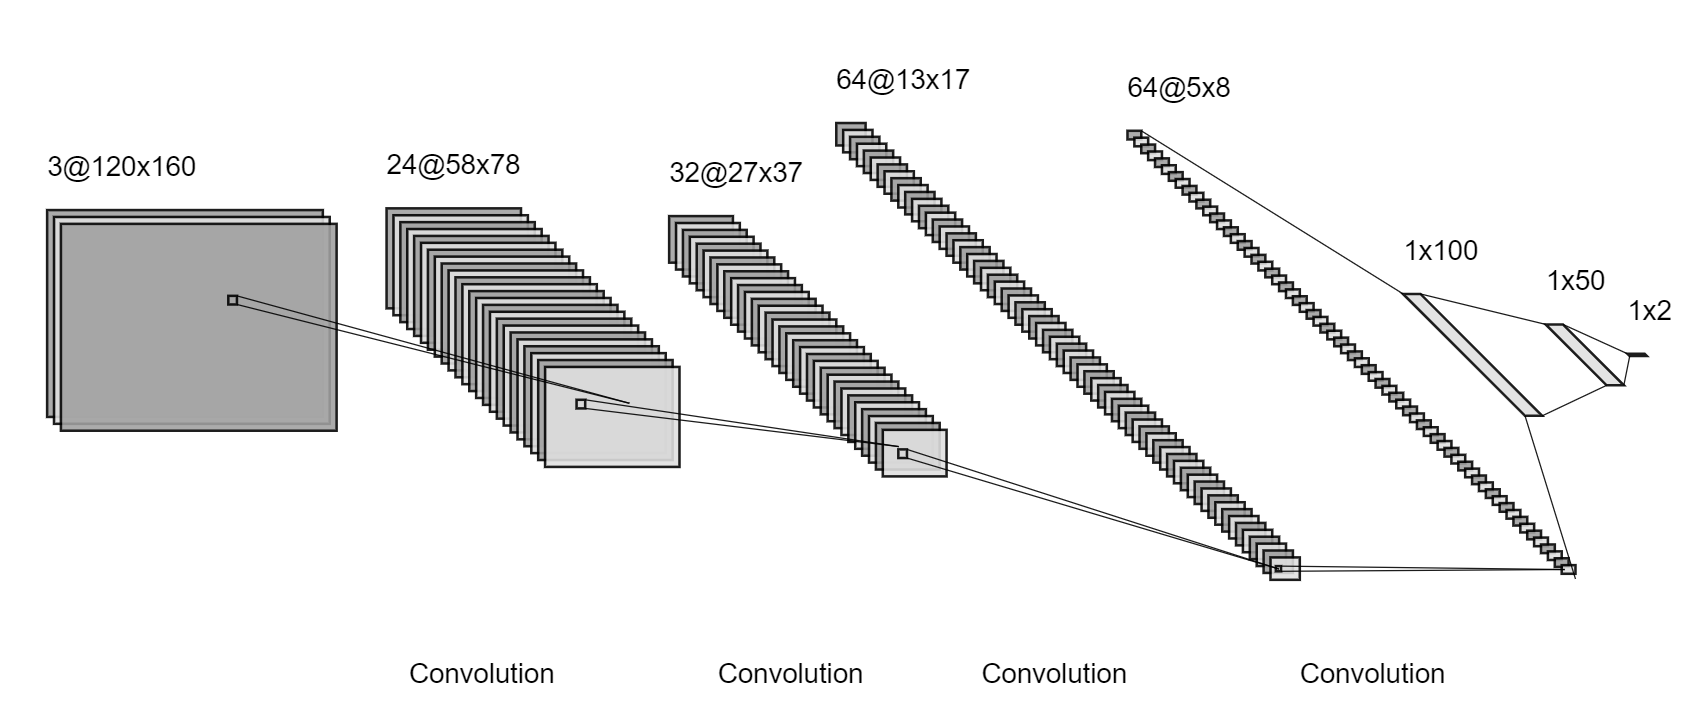
\includegraphics[width=0.5\textwidth]{ns.png}}
\caption{Model Structure.}
\label{ms}
\end{figure}

\begin{figure*}[t]
    \centering
    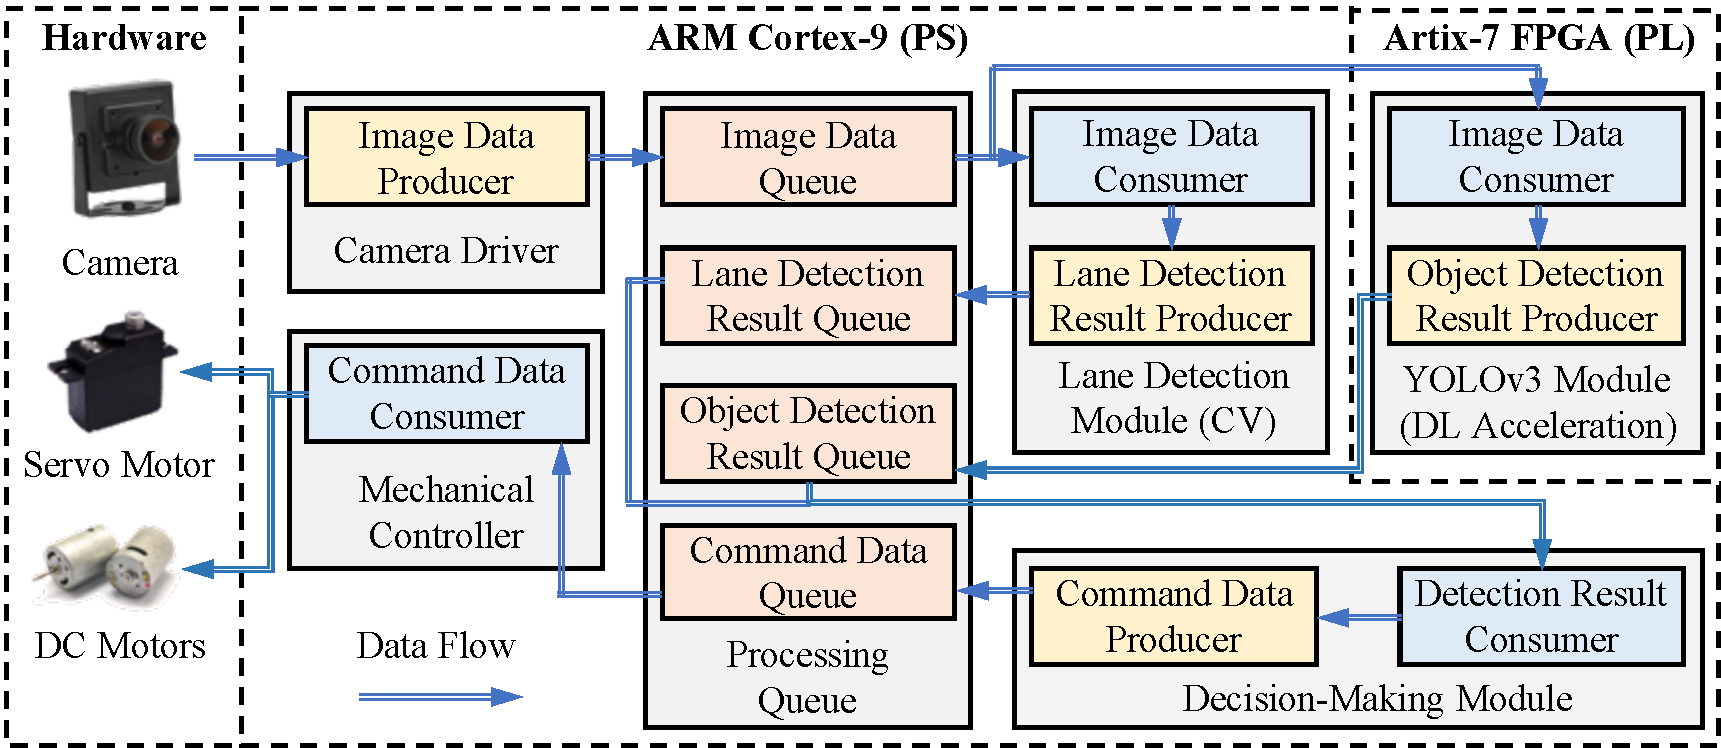
\includegraphics[width=5in]{traditional_autonomous_driving}
    \caption{Autonomous Driving using Traditional Methods.}
    \label{fig:traditional_autonomous_driving}
\end{figure*}

CNN layers extract features from the images taken by the car's front camera. Several fully connected layers follow the CNN layers, they finally extract the command information needed for auto-driving. The activation function we use is Relu. The last layer is a Softmax layer\cite{keras} for classification or a Dense layer for regression. Although the current model is not the perfect one, it's convenient to make changes and do optimizations to the model. Fig.~\ref{fig:end_to_end_autonomous_driving} shows the whole process.

First, you controls the car using your keyboard or whatever you like and save data from the car's sensors as training data. Or you just get the data from Internet or somewhere else. Second, after pre-process, you put the images you get as input to the AI model and the labels such as keyboard signals as the output. Train the model using TensorFlow until you get a satisfactory model. Third, you will use DNNDK\cite{dnndk} provided by Xilinx to do the compression and compilation and then copy the generated files to the car. Finally, the car is able to move by itself. It will be controlled by AI models. 

\begin{figure}[b]
    \centering
    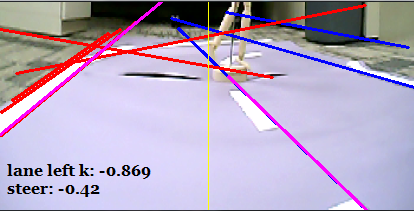
\includegraphics[width=3.5in]{lane_detect}
    \caption{Lane Detection.}
    \label{fig:lane_detection}
\end{figure}

\subsection{Autonomous Driving using traditional methods}
In the first case of AD we use an end-to-end model and in this one we will show you another way of doing AD. This time we will use computer vision methods to detect the road line and use classic YOLOv3 model to find objects.  

To detect road lane, we first use $5 \times 5$ Gaussian filter to remove the noise of the image. Then Canny edge detection\cite{canny1986computational} is applied to detect the edges of the image. Hough transform\cite{burns1986extracting} is employed to detect the lines of the image. Based on the orientation and relative position of detected lines, side line and stop line of the road are identified. To improve the robustness and accuracy of the algorithm, more techniques will be added to the algorithm, such as K-Means clustering\cite{selim1984k} for Hough lines, Kalman/Gabor filtering for sampled data, alternative IPM (inverse perspective mapping) lane detection method\cite{wang2014approach}.

The car will run following the lane of the road, Fig.~\ref{fig:lane_detection} shows the final lanes extracted from all detected lines. The yellow line marks the middle of the picture, the other lines are all lines we find in the photos. Among all the lanes we detected, we will choose one line for both left side and right side and they are painted purple. The red ones and blue ones are the rest. With these information, the car adjusts its direction and speed to the road. For example, in the picture the left lane chosen as the road line has a slope of $-0.869$ which is smaller than the slope datum, then the controller calculated a steer value $-0.42$ and that means to turn left.

\begin{figure}[b]
\centerline{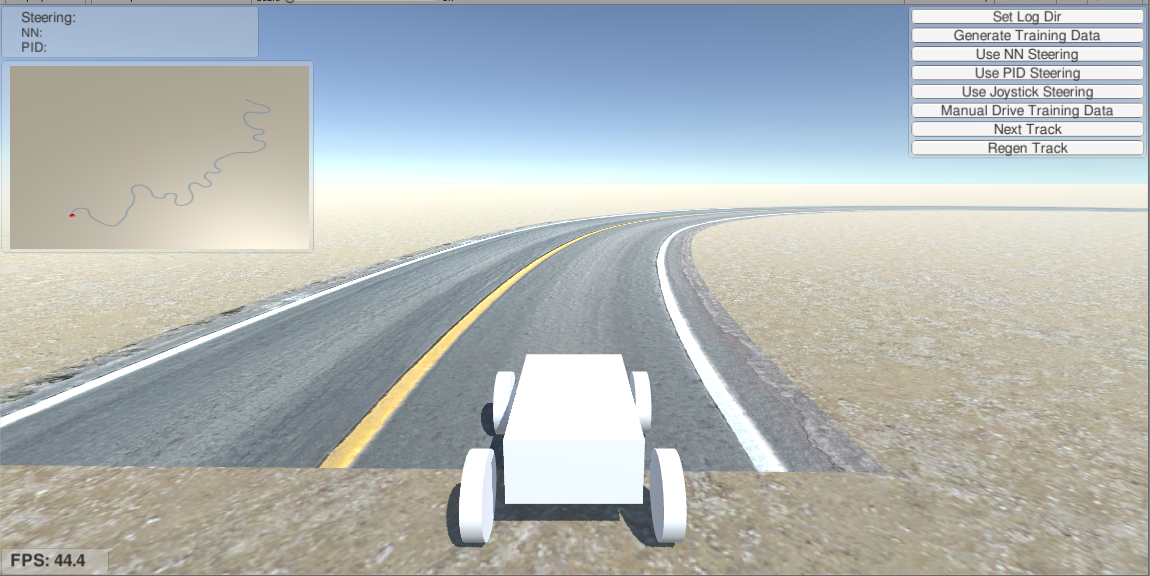
\includegraphics[width=0.5\textwidth]{simulator.png}}
\caption{Simulator Interface.}
\label{si}
\end{figure}

YOLOv3 is used to find objects like people or cars to help the car make decisions like braking to avoid a obstacle. The inference process will be accelerated by DNNDK to meet more stringent real-time requirement, also you could replace full YOLOv3 model with tiny YOLOv3 model to achieve faster inference speed.

Fig.~\ref{fig:traditional_autonomous_driving} shows the control process of this case, the taken images will be processed by both computer vision threads and YOLOv3 threads, this time they won't produce commands directly, instead the information they get will be used to make decisions. Finally, the commands will be generated by the decision maker.

\subsection{Simulator}
The simulator is a tool which helps users test their designs more efficiently. You see the interface of the simulator in Fig.~\ref{fig:lane_detection}. The simulator is based on sdsandbox\cite{sdsandbox} which is a simulator project for Donkey Car\cite{donkeycar}. As you see in the picture, the users use this simulator to collect training data and test their models. 

When testing, you should build a server, the server will receive sensor data from the client of the simulator and generate control messages according to these data. We have already built one example, the server will get images taken by simulator and handles them using the AI model trained before, then the model output control commands and these commands will be sent to the simulator.
It's also convenient for users to modify the source code of the simulator to define their own data format or control methods. However, users should be familiar with C\# and Unity3d if they would like to do so, and we provide coding tutorial manual to help.

\subsection{Lidar in ROS}
Due to the high impact of ROS, we make our platform able to support ROS projects. The version we use is ROS Melodic\cite{rosmelodic} which is mainly used in Ubuntu18.04. 

This time we show how to read LiDAR data and control the car using ROS. With Lidar data, the car is able to handle obstacle avoidance tasks and SLAM tasks whose basical technology is Lidar data processing.
The Lidar we use is LeiShen LS01D\cite{leishen}, LeiShen has already provided one ROS node for users to gain and publish Lidar data. We read the  laser point cloud data by subscribing the published topic. Also, it will be more visualized to use RViz\cite{rviz}, Fig.~\ref{ld} is one example.

\begin{figure}[b]
\centerline{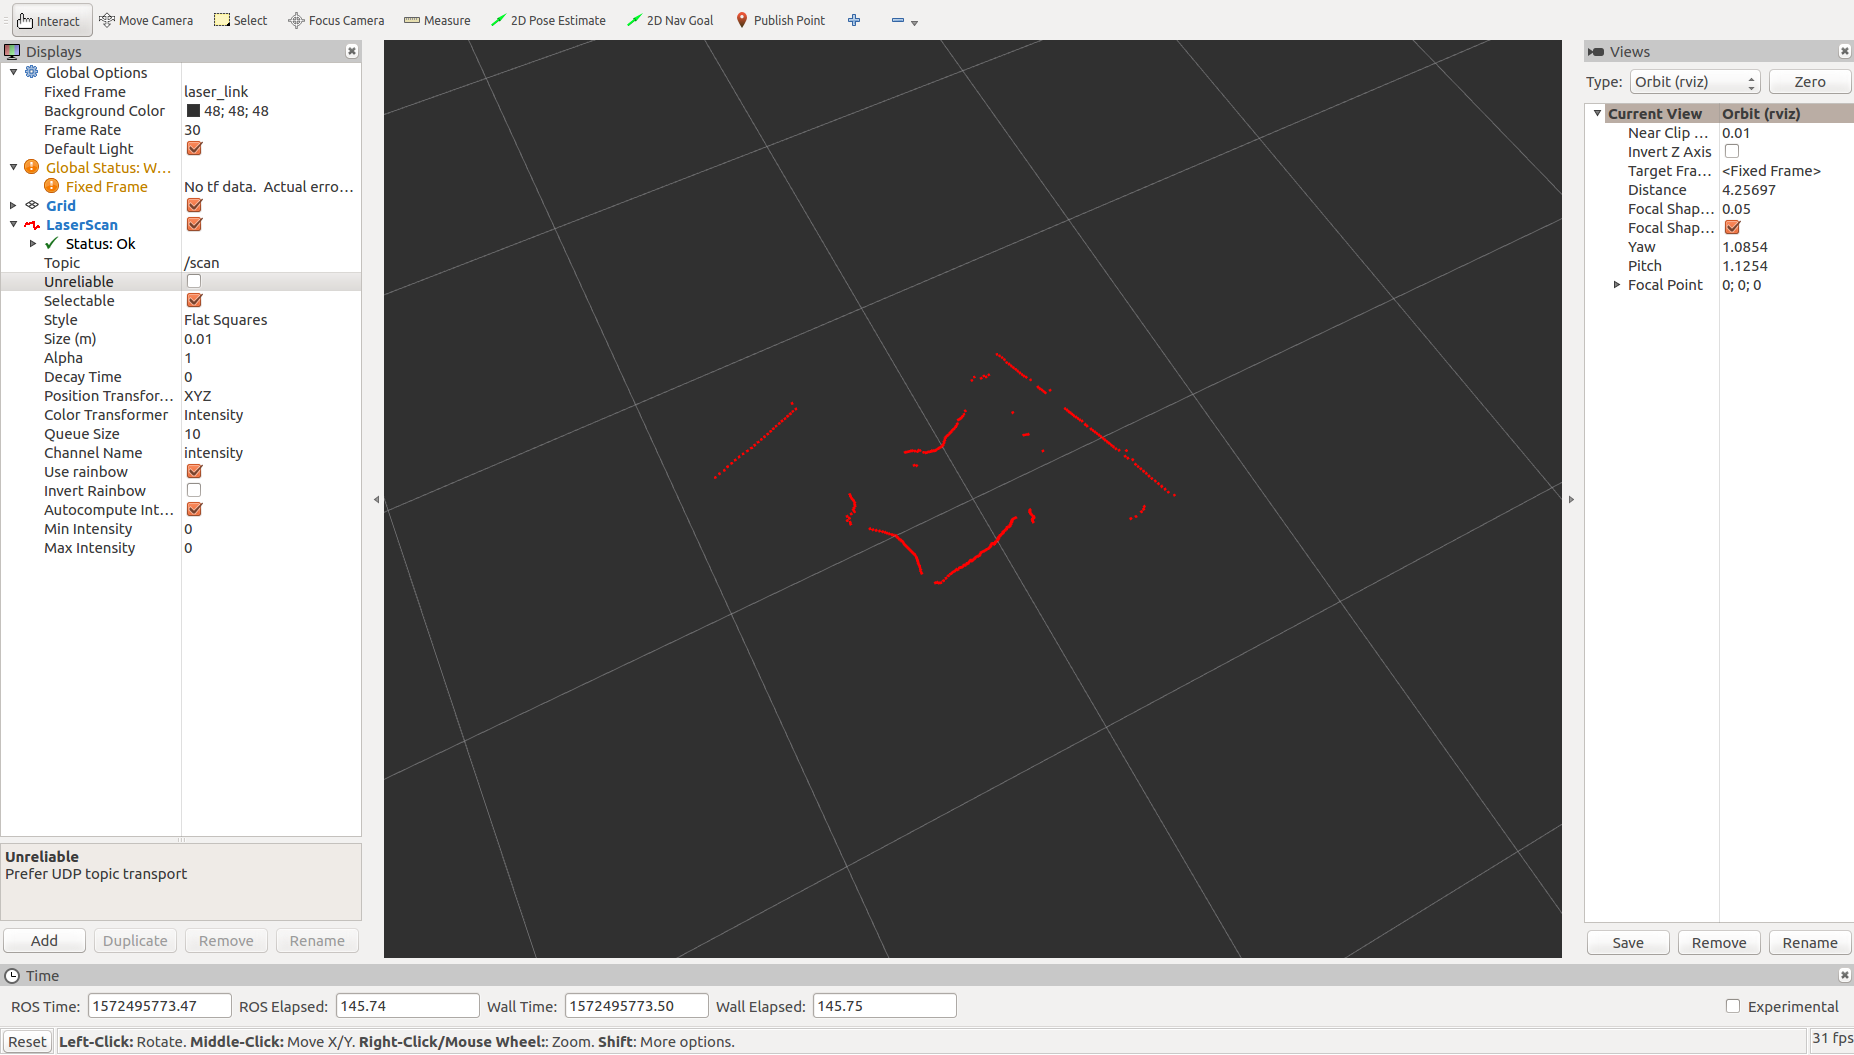
\includegraphics[width=0.5\textwidth]{laser.png}}
\caption{Lidar Data.}
\label{ld}
\end{figure}

The control node of the car is a transplantation of code from existing controller. It's easy to send control commands by publishing commands to corresponding topic. As we can see, it's easy for users to build their projects based on ROS in our platform. Since ROS is widely used, it's important that our platform helps users who want to try ROS.
\section{Conclusion}
In this paper, we present the design, implementation, characteristics and case studies of HydraMini, an affordable experimental research and education platform for autonomous driving. The platform is highly flexible and extensible, full stack, and easy-to-use. These three characteristics help users understand AD technology well and take full advantage of HydraMini. Students and researchers could use our platform for full-stack researches on algorithms, applications, system, mechanical control and hardware acceleration. We hope this platform helps users enjoy their research and learning process without paying much.

\bibliographystyle{IEEEtran}
\bibliography{ref}

\vspace{12pt}
\end{document}
